\chapter{Platforma sprzętowa i oprogramowanie wbudowane ESP32}
\label{ch:platforma_sprzetowa}

W rozbudowanych systemach badawczych typu \textit{Hardware-in-the-Loop} (HIL) fundamentem wiarygodności wyników jest urządzenie końcowe (węzeł pomiarowy).
Musi ono charakteryzować się zdolnością do deterministycznego przetwarzania gęstych strumieni danych sieciowych oraz precyzyjnego stemplowania pakietów w czasie (\textit{ang. timestamping}) w reżimie mikrosekundowym.
O ile logika orkiestracji eksperymentów została przeniesiona do warstwy skryptowej w języku Python, o tyle fizyczna akwizycja danych musi odbywać się na poziomie sprzętowym, pozbawionym narzutu systemów operacyjnych ogólnego przeznaczenia (GPOS).

W niniejszym projekcie funkcję tę powierzono mikrokontrolerowi \textbf{ESP32} firmy Espressif Systems.
Układ ten pełni w systemie podwójną rolę: z jednej strony utrzymuje wysokoczęstotliwościową pętlę komunikacji radiowej i przewodowej (\textit{Data Plane}), a z drugiej strony realizuje asynchroniczną wymianę komend z komputerem sterującym (\textit{Control Plane}).
Aby sprostać tak rygorystycznym wymaganiom czasowym, oprogramowanie wbudowane (\textit{ang. firmware}) napisane w języku C++ wymagało zastosowania zaawansowanych technik programistycznych oraz wykorzystania systemu czasu rzeczywistego FreeRTOS, który umożliwia równoległe wykonywanie wielu zadań na fizycznych rdzeniach procesora.

W niniejszym rozdziale zaprezentowano pełną architekturę stworzonego oprogramowania wbudowanego.
Omówiono wybór i konfigurację narzędzi programistycznych, zarządzanie rozszerzoną pamięcią operacyjną (PSRAM) w celu akwizycji dziesiątek tysięcy rekordów testowych oraz podział zadań na fizyczne rdzenie procesora z wykorzystaniem systemu czasu rzeczywistego.
Szczególną uwagę poświęcono również obiektowej architekturze oprogramowania opartej na wzorcu projektowym Strategia, która umożliwiła spójną, bezkolizyjną i wydajną obsługę wielu protokołów.

\section{Środowisko programistyczne - ekosystem PlatformIO}
\label{sec:ekosystem_platformio}

W tradycyjnym podejściu do programowania mikrokontrolerów popularnym środowiskiem jest Arduino IDE \cite{arduino_ide}, szczególnie na etapie nauki i prototypowania.
Jego istotną zaletą jest niski próg wejścia oraz wysoki poziom automatyzacji procesu przygotowania i wgrywania programu na płytkę.
Środowisko udostępnia między innymi mechanizmy zarządzania płytkami i bibliotekami, dzięki czemu rozpoczęcie pracy z mikrokontrolerem nie wymaga ręcznej konfiguracji całego łańcucha narzędzi.

Wraz ze wzrostem złożoności projektu większego znaczenia nabierają jednak możliwości organizacji procesu budowania, zarządzania zależnościami oraz jawnego definiowania konfiguracji sprzętowej i kompilatora.
W przypadku Arduino IDE część konfiguracji jest wykonywana za pośrednictwem ustawień środowiska.
Alternatywą jest otwartoźródłowy ekosystem PlatformIO \cite{platformio} - pozwala przenieść znaczną część tych informacji do konfiguracji projektu.
Zależności bibliotek mogą być deklarowane w pliku \texttt{platformio.ini}, podobnie jak informacje dotyczące platformy sprzętowej, używanego frameworka oraz parametrów procesu budowania.

Z tego względu jako główne środowisko programistyczne w niniejszym projekcie wykorzystano PlatformIO, zintegrowane z edytorem Visual Studio Code (tak jak pozostałe elementy projektu tworząc pełne rozwiązanie dostępne z poziomu jednej aplikacji (\textit{ang. AIO - All-in-One})).
Ekosystem ten obejmuje system budowania, zarządzanie pakietami i bibliotekami, monitor portu szeregowego, narzędzia debugowania oraz mechanizmy wspierające testowanie i analizę kodu.
Wykorzystanie tego rozwiązania pozwoliło na zastosowanie konfiguracji projektu, w której informacje dotyczące środowiska budowania, używanej płytki, frameworka, flag kompilatora oraz zależności są przechowywane w pliku \texttt{platformio.ini} (Listing \ref{lst:platformio_ini}).
Takie podejście zwiększa przejrzystość konfiguracji oraz ułatwia odtworzenie środowiska projektu na innej stacji roboczej.
PlatformIO umożliwia również określanie wersji zależności, co dodatkowo ogranicza ryzyko niekontrolowanych zmian środowiska podczas kolejnych kompilacji.

\begin{listing}[htbp]
    \caption{Deklaratywna konfiguracja środowiska kompilacji w ekosystemie PlatformIO (\texttt{platformio.ini}) \cite{espy_nexus_esp32_firmware}.}
    \label{lst:platformio_ini}
    \begin{minted}[fontsize=\footnotesize, linenos]{ini}
[env:esp-wrover-kit]
platform = espressif32
board = esp-wrover-kit
framework = arduino

monitor_speed = 921600
upload_port = COM3

lib_deps = links2004/WebSockets

build_flags = 
    ; Optimization for code execution speed
    -O3
    ; Disabling unnecessary system logs that slow down the processor
    -D CORE_DEBUG_LEVEL=0
    ; CRUCIAL FOR WROVER: Enabling external RAM (PSRAM)
    -D BOARD_HAS_PSRAM
    ; Hardware patch for stability during intensive memory transfers
    -mfix-esp32-psram-cache-issue


    ; --- Network configuration ---
    ; Setting the network mode: 
    ; - 0 for None,
    ; - 1 for Access Point (AP),
    ; - 2 for Station (STA), 
    -D NETWORK_MODE=2
    
    ; STA
    -D WIFI_STA_SSID=\"Your Wi-Fi SSID\"
    -D WIFI_STA_PASS=\"YourSuperSecretPassword\"
    
    ; AP
    -D WIFI_AP_SSID=\"ESPy_Nexus_AP\"
    -D WIFI_AP_PASS=\"YourSuperSecretPassword\"
    
    ; UDP
    -D UDP_PORT=8080

    ; TCP
    -D TCP_PORT=8080

    ; WebSocket
    -D WS_PORT=8080
\end{minted}
\end{listing}

Parametryzacja procesu kompilacji (\texttt{build\_flags}) została precyzyjnie dostosowana do rygorystycznych wymogów czasowych eksperymentów Hardware-in-the-Loop.
W środowisku tym zastosowano następujące krytyczne dyrektywy:

\begin{itemize}
    \item \texttt{-O3} - agresywna flaga kompilatora GCC (ang. \textit{Level 3 Optimization}).
          W standardowych projektach stosuje się optymalizację pod kątem redukcji rozmiaru pliku wynikowego (\texttt{-Os}).
          W projektowanym węźle pomiarowym priorytetem jest jednak uzyskanie absolutnie najwyższej szybkości wykonywania instrukcji, co bezpośrednio przekłada się na redukcję narzutu obliczeniowego przy precyzyjnym stemplowaniu czasowym (mikrosekundowym).
    \item \texttt{-D CORE\_DEBUG\_LEVEL=0} - całkowite wyłączenie systemowych logów diagnostycznych rdzenia ESP32.
          Wypisywanie informacji z użyciem wbudowanego interfejsu UART jest operacją wysoce blokującą.
          Jakikolwiek nieoczekiwany zrzut informacji z bibliotek Wi-Fi w trakcie trwania szybkiej transmisji uszkodziłby rygorystyczne ramy czasowe pętli HIL, a w przypadku wariantu komunikacji bezpośredniej (\texttt{SERIAL\_BIN} lub \texttt{SERIAL\_STR}) doprowadziłby do krytycznej korupcji transportowanych strumieni binarnych.
    \item \texttt{-D BOARD\_HAS\_PSRAM} oraz \texttt{-mfix-esp32-psram-cache-issue} - aktywacja i sprzętowe łatanie magistrali zewnętrznej pamięci RAM.
          Dyrektywy te są fundamentalne dla funkcjonowania aplikacji, pozwalając na zaalokowanie buforów przekraczających fizyczne możliwości mikrokontrolera.
    \item \texttt{-D NETWORK\_MODE} - własna dyrektywa preprocesora C++, umożliwiająca kompilację warunkową kodu źródłowego (\#ifdef).
          Zapewnia ona łatwą rekonfigurację topologii radiowej (tworzenie własnej sieci punktu dostępowego lub podłączenie do zewnętrznego routera) bez konieczności ingerencji w logikę plików \texttt{.cpp}.
\end{itemize}

\section{Architektura mikrokontrolera ESP32}
\label{sec:architektura_esp32}

W projektowanym systemie jako jednostkę obliczeniową węzła pomiarowego wykorzystano płytkę rozwojową \textbf{ESP32-DevKitC-VIE} firmy Espressif (Rys. \ref{fig:esp32-devkitC-vie.png}).
Oznaczenie tego wariantu sprzętowego należy rozpatrywać na kilku poziomach architektonicznych - ESP32 to nazwa podstawowej rodziny układów, natomiast DevKitC-VIE to nazwa samej płytki bazowej (ewaluacyjnej) posiadającej zarówno wbudowaną antenę drukowaną na laminacie (\textit{ang. PCB antenna}), jak i możliwość współpracy z zewnętrzną anteną poprzez dedykowane złącze.
Moduł lutowany jest powierzchniowo na PCB, gdzie dodatkowo wyprowadzone są piny GPIO układu umożliwiające korzystanie z przerwań sprzętowych i bogatych układów peryferyjnych, a także integruje obwody zasilania i konwerter USB-UART, znacząco ułatwiając programowanie układu (Rys. \ref{fig:esp32-devkitC-v4-pinout.png}).

\begin{figure}[htbp]
    \centering
    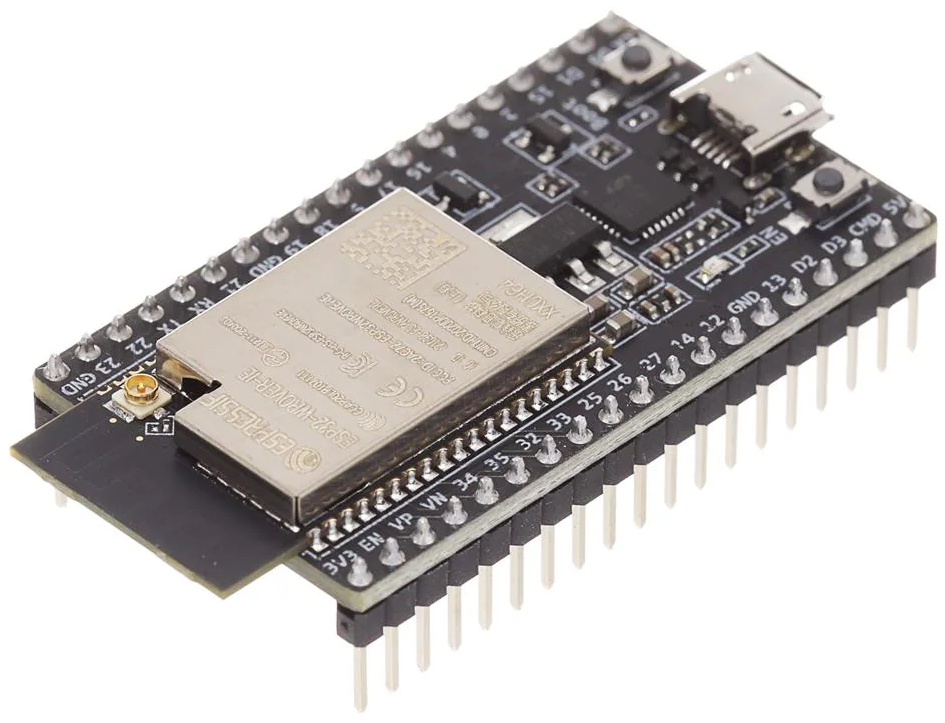
\includegraphics[width=0.8\textwidth]{images/esp32/ESP32-DevKitC-VIE.png}
    \caption{Mikrokontroler ESP32-DevKitC-VIE \cite{esp32_mouser}.}
    \label{fig:esp32-devkitC-vie.png}
\end{figure}

\begin{figure}[htbp]
    \centering
    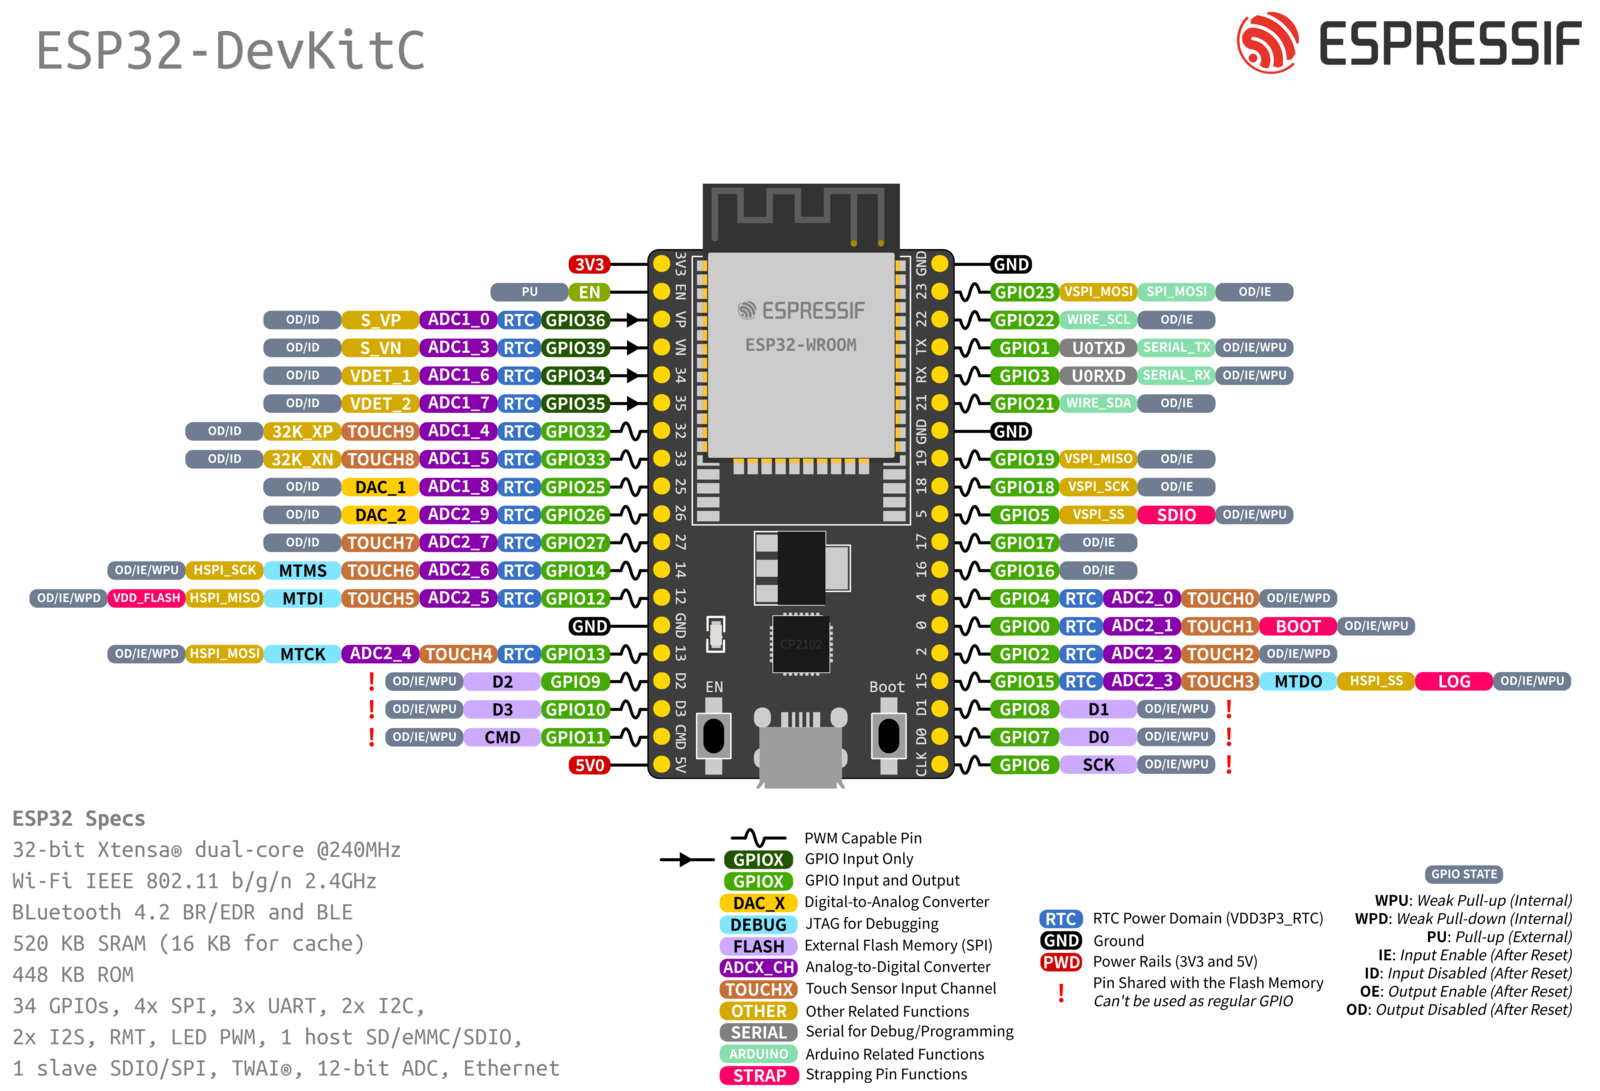
\includegraphics[width=\textwidth]{images/esp32/esp32-devkitC-v4-pinout.png}
    \caption{Płytka rozwojowa ESP32-DevKitC-V4 - pinout \cite{esp32_pinout}.}
    \label{fig:esp32-devkitC-v4-pinout.png}
\end{figure}

Mikrokontrolery z rodziny ESP32 oparte na architekturze Xtensa oferują gigantyczną przewagę obliczeniową i komunikacyjną nad klasycznymi układami stosowanymi w typowych projektach edukacyjnych, co czyni je optymalnym wyborem dla zaawansowanych systemów czasu rzeczywistego, a także filarem wielu rozwiązań SmartHome.
Szczegółowe zestawienie parametrów sprzętowych zastosowanego modułu, w odniesieniu do referencyjnej, popularnej platformy Arduino UNO R3, zaprezentowano w tabeli \ref{tab:esp32_vs_uno}.

\begin{table}[htbp]
    \centering
    \caption{Porównanie parametrów ESP32-DevKitC-VIE \cite{esp32} oraz referencyjnego Arduino UNO R3 \cite{arduino_uno_rev3}.}
    \label{tab:esp32_vs_uno}
    \begin{tabular}{|l|c|c|}
        \hline
        \textbf{Parametr}        & \textbf{ESP32-DevKitC-VIE}    & \textbf{Arduino UNO R3} \\
        \hline
        Układ bazowy             & ESP32-WROVER-IE               & ATmega328P              \\
        \hline
        Architektura CPU         & 32-bit                        & 8-bit                   \\
        \hline
        Liczba rdzeni            & 2                             & 1                       \\
        \hline
        Częstotliwość taktowania & do 240 MHz                    & 16 MHz                  \\
        \hline
        Pamięć SRAM              & 520 KB                        & 2 KB                    \\
        \hline
        Pamięć Flash             & 4 MB                          & 32 KB                   \\
        \hline
        Pamięć zewnętrzna PSRAM  & 8 MB                          & brak                    \\
        \hline
        Interfejs Wi-Fi          & 802.11 b/g/n 2,4 GHz          & brak                    \\
        \hline
        Interfejs Bluetooth      & Bluetooth 4.2 BR/EDR oraz BLE & brak                    \\
        \hline
        Napięcie logiki układu   & 3,3 V                         & 5 V                     \\
        \hline
    \end{tabular}
\end{table}

Głównym wyzwaniem programistycznym w kontekście warstwy sprzętowej była konieczność lokalnego buforowania gigantycznej liczby zdarzeń sieciowych.
Architektura systemu zakłada zgromadzenie \texttt{MAX\_RECORDS = 50000} pomiarów przed ich ostatecznym zrzutem do warstwy analitycznej.
Mimo że ESP32 oferuje wielokrotnie więcej natywnej pamięci SRAM (520 KB) niż układy takie jak ATmega328P, znaczna jej część jest rezerwowana przez system operacyjny FreeRTOS, stos sieciowy protokołu TCP/IP (lwIP) oraz sterowniki Wi-Fi.
Próba zaalokowania tablicy pomiarowej w wewnętrznej pamięci SRAM skutkowałaby przepełnieniem sterty (\textit{ang. Heap Overflow}) i restartem układu z użyciem mechanizmu zabezpieczającego \textit{Watchdog}.

\subsection{Zarządzanie pamięcią zewnętrzną PSRAM}
\label{psram}

Problem ten rozwiązano dzięki obecności wspominanej pamięci PSRAM.
Jak zaprezentowano na Listingu \ref{lst:psram_malloc}, program przed uruchomieniem maszyny stanów weryfikuje sprzętową dostępność zewnętrznego modułu pamięci za pomocą metody \texttt{psramFound()}.
Następnie, wykorzystując wywołanie \texttt{ps\_malloc()}, wymusza na wbudowanym alokatorze zlokalizowanie bufora wynikowego (\texttt{resultBuffer}) bezpośrednio w układzie PSRAM.
Chroni to szybką pamięć wewnętrzną przed defragmentacją, pozostawiając ją do wyłącznej dyspozycji krytycznych czasowo procesów komunikacyjnych.

\begin{listing}[htbp]
    \caption{Wymuszona alokacja bufora pomiarowego w pamięci PSRAM (\texttt{main.cpp}) \cite{espy_nexus_esp32_firmware}.}
    \label{lst:psram_malloc}
    \begin{minted}[fontsize=\footnotesize, linenos]{cpp}
const uint32_t MAX_RECORDS = 50000;
TestRecord *resultBuffer = nullptr;

// ...
  // PSRAM allocation for result buffer
  if (psramFound())
  {
    Serial.printf("Allocating PSRAM for %u records...\n", MAX_RECORDS);
    resultBuffer = (TestRecord *)ps_malloc(MAX_RECORDS * sizeof(TestRecord));

    if (resultBuffer != nullptr)
    {
      Serial.printf("OK! Allocated %u bytes.\n", MAX_RECORDS * sizeof(TestRecord));
    }
    else
    {
      Serial.println("FATAL ERROR: PSRAM allocation failed!");
      while (1)
        ;
    }
  }
\end{minted}
\end{listing}

W systemach wbudowanych o ograniczonych zasobach, kompresja i wyrównanie pamięci na poziomie kompilatora odgrywa niebagatelną rolę.
Standardową praktyką kompilatorów C/C++ jest wyrównywanie struktur w pamięci (\textit{ang. Data Structure Alignment}) do granic słowa maszynowego (z reguły 4 lub 8 bajtów), co przyspiesza instrukcje odczytu, lecz powoduje wstawienie niewidocznych, pustych bajtów buforujących (ang.
\textit{Padding}).
Struktura rekordu pomiarowego zdefiniowana w systemie \textit{ESPy-Nexus} składa się z 32-bitowego identyfikatora pakietu (\texttt{uint32\_t} - 4 bajty) oraz 64-bitowego stempla czasowego (\texttt{int64\_t} - 8 bajtów).
Ze względu na narzucone wyrównanie do typu 64-bitowego, kompilator natywnie wstawiłby 4 bajty pustego \textit{paddingu} pomiędzy zmiennymi, rozszerzając fizyczny rozmiar struktury z matematycznych 12 do 16 bajtów.

Narzut rzędu 4 bajtów, pomnożony przez założone 50 000 iteracji pomiarowych, skutkowałby nieuzasadnioną stratą niemal 200 KB cennego obszaru operacyjnego.
Aby wyeliminować to zjawisko, definicję struktury obarczono specjalną dyrektywą środowiska GCC - \texttt{\_\_attribute\_\_((packed))} (Listing \ref{lst:packed_struct}).
Atrybut ten wymusza na kompilatorze bezwzględną eliminację wyrównywania pamięci, co gwarantuje, że wpis waży dokładnie 12 bajtów (\texttt{sizeof(TestRecord)}).
Umożliwiło to zoptymalizowanie alokacji w układzie PSRAM oraz znaczące zredukowanie ilości danych przesyłanych kanałem szeregowym (UART) na etapie zrzutu wyników do komputera sterującego.

\begin{listing}[htbp]
    \caption{Struktura \texttt{TestRecord} - eliminacja pustych bajtów wyrównania w strukturze pomiarowej (\texttt{TestRecord.h}) \cite{espy_nexus_esp32_firmware}.}
    \label{lst:packed_struct}
    \begin{minted}[fontsize=\footnotesize, linenos]{cpp}
#pragma once
#include <Arduino.h>

// __attribute__((packed)) removes hardware padding (empty alignment bytes).
struct __attribute__((packed)) TestRecord
{
    uint32_t packet_id;        // 4 bytes
    int64_t esp_timestamp_us;  // 8 bytes
};
// Total size of the new struct: 12 bytes
\end{minted}
\end{listing}

\section{Architektura wielowątkowa w systemie czasu rzeczywistego (FreeRTOS)}
\label{sec:freertos_architektura}

Klasyczny paradygmat programowania mikrokontrolerów, spopularyzowany przez środowisko Arduino, opiera się na wykonywaniu instrukcji w pojedynczej, nieskończonej pętli głównej (\texttt{loop()}) poprzedzonej przez funkcję inicjalizacyjną (\texttt{setup()}).
W zaawansowanych systemach pomiarowych, takich jak węzeł HIL, podejście jednowątkowe jest niewystarczające.
Konieczność jednoczesnego nasłuchiwania interfejsu sterującego (UART), zarządzania maszyną stanów oraz dekodowania gęstego strumienia danych sieciowych w jednym wątku doprowadziłoby do drastycznych opóźnień (zjawisko \textit{Jitteru} systemowego) i gubienia pakietów.

Aby zagwarantować determinizm czasowy, oprogramowanie układu ESP32 zostało oparte na systemie operacyjnym czasu rzeczywistego \textbf{FreeRTOS}, natywnie wspieranym przez układ Espressif.
Architektura ta pozwoliła na całkowite porzucenie klasycznej pętli \texttt{loop()}, w której wnętrzu wywoływana jest jedynie funkcja \texttt{vTaskDelete(NULL)}, co definitywnie usuwa domyślny wątek środowiska Arduino z pamięci operacyjnej i oddaje pełną kontrolę nad procesorem zaplanowanym, dedykowanym zadaniom (\textit{ang. Tasks}).

\subsection{Podział obowiązków i przypisanie do rdzeni}
Dwurdzeniowa architektura procesora Xtensa LX6 umożliwiła rygorystyczną separację procesów komunikacyjnych (\textit{Control Plane}) od krytycznych procesów pomiarowych (\textit{Data Plane}).
Wykorzystując specyficzną dla układów ESP32 funkcję \texttt{xTaskCreatePinnedToCore()}, rozdzielono i przypięto zadania do konkretnych fizycznych rdzeni procesora (Listing \ref{lst:freertos_tasks}):

\begin{itemize}
    \item \textbf{Rdzeń 0 (systemowy - PRO\_CPU):}
          tradycyjnie obciążony obsługą stosu radiowego (Wi-Fi/Bluetooth).
          Przypisano do niego dwa zadania administracyjne:
          \begin{itemize}
              \item \texttt{UartListenerTask} (Priorytet 2): niskopoziomowy proces asynchronicznie nasłuchujący bufora interfejsu szeregowego.
                    Odbiera on znaki od komputera sterującego (skryptów Python) i składa je w kompletne ramki tekstowe.
              \item \texttt{ControlTask} (Priorytet 1): wątek maszyny stanów.
                    Odpowiada za parsowanie komend (np. \texttt{START\_TCP}, \texttt{STOP}, \texttt{GET\_DATA}) oraz dynamiczną inicjalizację odpowiednich obiektów warstwy pomiarowej.
                    Niższy priorytet gwarantuje, że parsowanie poleceń nie zablokuje procesu odczytu z portu UART.
          \end{itemize}
    \item \textbf{Rdzeń 1 (aplikacyjny - APP\_CPU):}
          całkowicie odizolowany od warstwy sterującej.
          Przypięto do niego wyłącznie jedno, krytyczne zadanie pomiarowe: \texttt{DataTask}.
          Otrzymało ono absolutnie \textbf{maksymalny priorytet systemowy} (\texttt{configMAX\_PRIORITIES - 1}).
          Oznacza to, że proces pobierania danych i stemplowania ich w czasie (\textit{timestamping}) nie może zostać wywłaszczony (\textit{ang. preempted}) przez żadne inne zadanie aplikacyjne.
          Gwarantuje to najwyższą możliwą precyzję pomiaru opóźnień HIL, eliminując zakłócenia wynikające z przełączania kontekstu (\textit{ang. Context Switching}).
\end{itemize}

\begin{listing}[htbp]
    \caption{Porzucenie pętli głównej i utworzenie rygorystycznych wątków systemowych przypiętych do rdzeni procesora (\texttt{main.cpp}) \cite{espy_nexus_esp32_firmware}.}
    \label{lst:freertos_tasks}
    \begin{minted}[fontsize=\footnotesize, linenos]{cpp}
void setup()
{
  // [...] Inicjalizacja środowiska w funkcji setup()

  // Utworzenie bezpiecznej kolejki kontrolnej
  // Create control queue and tasks
  controlQueue = xQueueCreate(10, sizeof(char[32]));

  // Rdzeń 0: Zadania nasłuchujące i sterujące eksperymentem
  xTaskCreatePinnedToCore(
      uartListenerTask, "UartListener", 2048, NULL, 2, NULL, 0);

  xTaskCreatePinnedToCore(
      controlPlaneTask, "ControlTask", 4096, NULL, 1, NULL, 0);

  // Rdzeń 1: Ekstremalnie priorytetowe zadanie akwizycji danych
  xTaskCreatePinnedToCore(
      dataPlaneTask, "DataTask", 8192, NULL, configMAX_PRIORITIES - 1, NULL, 1);

  Serial.println("\n--- System Ready ---");
}

void loop()
{
  // Usunięcie domyślnego wątku Arduino - pełna kontrola przekazana do FreeRTOS
  vTaskDelete(NULL);
}
\end{minted}
\end{listing}

\subsection{Komunikacja międzyprocesowa (IPC) i synchronizacja}
Oddzielenie wątków na różnych rdzeniach procesora stwarza ryzyko wystąpienia tzw. wyścigów (\textit{ang. Race Conditions}) przy próbie jednoczesnego dostępu do współdzielonych zasobów.
W systemie zrezygnowano z używania niestabilnych, globalnych flag bitowych na rzecz natywnego mechanizmu komunikacji międzyprocesowej (\textit{ang. IPC - Inter-Process Communication}) środowiska FreeRTOS - kolejek (\texttt{QueueHandle\_t}).

Jak zaprezentowano na Listingu \ref{lst:freertos_queue}, po zdekodowaniu pełnej komendy, wątek \texttt{uartListenerTask} asynchronicznie wypycha dane do kolejki \texttt{controlQueue} z użyciem funkcji \texttt{xQueueSend()}.
Z kolei wątek \texttt{controlPlaneTask} używa funkcji \texttt{xQueueReceive()} z parametrem \texttt{portMAX\_DELAY}.
Powoduje to natychmiastowe zablokowanie zadania (zdjęcie go z procesora) do momentu fizycznego pojawienia się nowej komendy w kolejce.
W efekcie, wątek kontrolny nie zużywa cykli obliczeniowych procesora na aktywne oczekiwanie (\textit{ang. busy waiting}), pozostając w uśpieniu i budząc się wyłącznie w chwili odebrania zlecenia z zewnątrz, co drastycznie optymalizuje wykorzystanie zasobów mikrokontrolera.

\begin{listing}[htbp]
    \caption{Mechanizm bezkolizyjnej komunikacji IPC pomiędzy rdzeniami za pomocą kolejek systemowych (\texttt{main.cpp}) \cite{espy_nexus_esp32_firmware}.}
    \label{lst:freertos_queue}
    \begin{minted}[fontsize=\footnotesize, linenos]{cpp}
void uartListenerTask(void *pvParameters)
{
  char rx_buffer[32];
  // [...] Parsowanie pojedynczych znaków z UART
          rx_buffer[rx_index] = '\0';
          // Wysłanie zdekodowanej komendy do kolejki IPC (nieblokująco)
          xQueueSend(controlQueue, &rx_buffer, 0); 
  // [...]
}

void controlPlaneTask(void *pvParameters)
{
  char cmd[32];
  for (;;)
  {
    // Zadanie pozostaje zablokowane (uśpione) do momentu pojawienia się komendy
    if (xQueueReceive(controlQueue, &cmd, portMAX_DELAY) == pdPASS)
    {
      String command(cmd);
      command.trim();

      if (command.startsWith("START_")) {
          // Logika inicjalizacji warstwy pomiarowej
      }
      // [...]
    }
  }
}
\end{minted}
\end{listing}

\section{Wzorzec projektowy Strategia}
\label{sec:wzorzec_strategia}

Oprogramowanie węzła badawczego wymagało zaimplementowania obsługi wielu skrajnie różnych protokołów komunikacyjnych: strumieniowego protokołu TCP, bezpołączeniowego UDP, zorientowanych na ramki WebSockets oraz dwóch wariantów transmisji szeregowej (binarnej i tekstowej).
Klasyczne, strukturalne podejście do tego problemu skutkowałoby stworzeniem monolitycznej pętli głównej, przepełnionej instrukcjami warunkowymi (\texttt{switch}/\texttt{if-else}) sprawdzającymi aktualny tryb pracy.
Taka architektura jest trudna w utrzymaniu, podatna na błędy i łamie fundamentalną zasadę otwarte-zamknięte (\textit{ang. Open/Closed Principle}) z SOLID \cite{solid}, ponieważ dodanie nowego protokołu wymagałoby modyfikacji krytycznego jądra systemu skutkując powstawaniem spaghetti code.

Aby zagwarantować najwyższą jakość architektury oprogramowania warstwę akwizycji danych zrealizowano w oparciu o obiektowy wzorzec projektowy \textbf{Strategia} (\textit{Strategy Pattern}).
Pozwala on na zdefiniowanie rodziny algorytmów (w tym przypadku protokołów), hermetyzację każdego z nich w oddzielnej klasie i umożliwienie ich swobodnego, dynamicznego podmieniania w trakcie działania programu.

\subsection{Abstrakcyjny interfejs komunikacyjny}
\label{sec:abstrakcyjny_interfejs_komunikacyjny}

Fundamentem wdrożonego wzorca jest wirtualna klasa bazowa \texttt{IDataPlane} (Listing \ref{lst:idataplane}), pełniąca rolę kontraktu (interfejsu) pomiędzy maszyną stanów, a konkretnymi implementacjami protokołów.
Zdefiniowano w niej trzy czysto wirtualne metody:
\begin{itemize}
    \item \texttt{begin()} - inicjalizacja gniazd i buforów,
    \item \texttt{process()} - główny algorytm pobierający i dekodujący pakiety,
    \item \texttt{end()} - bezpieczne zamykanie połączeń.
\end{itemize}

Obecność wirtualnego destruktora (\texttt{virtual \textasciitilde IDataPlane()}) jest rygorystycznym wymogiem języka C++ zapobiegającym wyciekom pamięci w przypadku polimorficznego usuwania obiektów pochodnych.

\begin{listing}[htbp]
    \caption{Definicja abstrakcyjnego interfejsu warstwy danych wymuszającego rygorystyczny kontrakt (\texttt{IDataPlane.h}) \cite{espy_nexus_esp32_firmware}.}
    \label{lst:idataplane}
    \begin{minted}[fontsize=\footnotesize, linenos]{cpp}
#pragma once
#include <Arduino.h>
#include <freertos/FreeRTOS.h>
#include <freertos/queue.h>
#include "TestRecord.h"

class IDataPlane
{
public:
    virtual ~IDataPlane() = default;

    virtual bool begin() = 0;
    virtual void process(TestRecord *buffer, volatile uint32_t &recordCount, 
        uint32_t maxRecords, QueueHandle_t ctrlQueue) = 0;
    virtual void end() = 0;
};
\end{minted}
\end{listing}

Każdy z obsługiwanych protokołów otrzymał własną, wyizolowaną klasę dziedziczącą (np. \texttt{TcpDataPlane}, \texttt{SerialBinDataPlane}), która przesłania (\textit{ang. override}) metody interfejsu, implementując specyficzną dla siebie logikę obsługi sprzętowej.

\subsection{Polimorfizm protokołów w głównym wątku pomiarowym}
\label{sec:polimorfizm_proces}

Zastosowanie interfejsu pozwoliło na drastyczne uproszczenie wielowątkowej architektury w głównym pliku aplikacji (\texttt{main.cpp}).
Zadeklarowano globalny wskaźnik polimorficzny \texttt{IDataPlane *currentDataPlane}, który w danej chwili może wskazywać na dowolny z zainstancjowanych protokołów.

Gdy wątek zarządzający (\texttt{ControlTask}) odbierze od środowiska Python polecenie rozpoczęcia eksperymentu (np. \texttt{START\_TCP}), dokonuje on przypisania adresu konkretnego obiektu do wskaźnika bazowego (\texttt{currentDataPlane = \&tcpDataPlane}) oraz wywołuje jego metodę inicjalizacyjną.
Dzięki mechanizmowi \textbf{późnego wiązania} (\textit{ang. Late Binding / Dynamic Dispatch}) główny wątek pomiarowy (\texttt{DataTask}) przypięty do rdzenia aplikacyjnego pozostaje całkowicie niezależny od aktualnie wybranego protokołu (Listing \ref{lst:polimorfizm_proces}).

Wykonuje on w pętli wyłącznie polimorficzne wywołanie dziedziczonej metody \texttt{process()}.
Dzięki takiej abstrakcji wątek pomiarowy nie jest powiązany z aktualnie działającym protokołem - nie musi wiedzieć, czy aktualnie czyta z gniazda WebSocket, czy z portu szeregowego.
Takie podejście maksymalizuje czytelność kodu, eliminuje narzut instrukcji warunkowych w krytycznej pętli czasowej i pozwala na błyskawiczne dodanie obsługi nowych protokołów w przyszłości bez konieczności modyfikowania jądra systemu.

\begin{listing}[htbp]
    \caption{Wykorzystanie polimorfizmu do bezwarunkowego wykonywania procesów sieciowych w głównym wątku pomiarowym (\texttt{main.cpp}) \cite{espy_nexus_esp32_firmware}.}
    \label{lst:polimorfizm_proces}
    \begin{minted}[fontsize=\footnotesize, linenos]{cpp}
// Globalny wskaźnik do abstrakcyjnego interfejsu
IDataPlane *currentDataPlane = nullptr;

// Ekstremalnie zoptymalizowany wątek pomiarowy (Rdzeń 1)
void dataPlaneTask(void *pvParameters)
{
  for (;;)
  {
    // Brak instrukcji switch/if-else sprawdzających protokół.
    // Metoda wirtualna rozwiązywana jest w locie (Late Binding).
    if (isTestRunning && currentDataPlane != nullptr)
    {
      currentDataPlane->process(resultBuffer, recordCount, 
                                MAX_RECORDS, controlQueue);
    }
    taskYIELD();
  }
}

// Fragment wątku sterującego (Rdzeń 0) obsługujący zmianę strategii
if (protocol == "TCP")
{
  // Wstrzyknięcie strategii dla TCP
  currentDataPlane = &tcpDataPlane;
  initSuccess = currentDataPlane->begin();
  serialPortOwnedByDataPlane = false;
}
else if (protocol == "SERIAL_BIN")
{
  // Wstrzyknięcie strategii dla binarnego portu szeregowego
  currentDataPlane = &serialBinDataPlane;
  initSuccess = currentDataPlane->begin();
  serialPortOwnedByDataPlane = true;
}
\end{minted}
\end{listing}

\section{Implementacja interfejsów komunikacyjnych}
\label{sec:interfejsy_komunikacyjne}

Zaimplementowanie abstrakcyjnego interfejsu \texttt{IDataPlane} pozwoliło na zdefiniowanie pięciu niezależnych mechanizmów akwizycji danych: UDP, TCP, WebSockets oraz dwóch wariantów interfejsu szeregowego (tekstowego i binarnego).
Każdy z tych protokołów charakteryzuje się odmiennym sposobem dostarczania ładunku (\textit{ang. payload}), co wymagało zastosowania dedykowanych strategii buforowania oraz dekodowania, przy jednoczesnym zachowaniu rygoru czasowego HIL.

Protokoły oparte na datagramach (takie jak UDP, czy ramki WebSockets) dostarczają do mikrokontrolera kompletne, odseparowane od siebie pakiety informacji.
Z tego względu wyodrębnienie pojedynczego pomiaru sprowadza się do odczytania bufora systemowego.
Zupełnie inaczej sytuacja wygląda w przypadku protokołu TCP oraz interfejsu UART.
Oba te standardy to tzw. protokoły strumieniowe (\textit{ang. Stream-oriented protocols}), które nie zachowują granic pomiędzy wysłanymi pakietami.
Mikrokontroler otrzymuje ciągły potok bajtów i musi samodzielnie określić, w którym miejscu kończy się jedna ramka danych, a zaczyna kolejna.

W przypadku protokołów tekstowych (np. \texttt{SerialStrDataPlane}), problem ten rozwiązuje się trywialnie poprzez wykorzystanie znaku nowej linii (\texttt{\char`\\n}) jako separator.
Podejście to jest jednak niewydajne - konwersja liczb na tekst (ASCII) i ich powrotne parsowanie (np. funkcją \texttt{atoi}) niepotrzebnie obciąża procesor, a same pakiety zajmują wielokrotnie więcej miejsca.

Aby zmaksymalizować przepustowość, węzeł \textit{ESPy-Nexus} wykorzystuje transmisję w 100\% binarną (\texttt{SerialBinDataPlane}, \texttt{TcpDataPlane}).
Wynika z tego jednak krytyczny problem: jeśli jako separatora użyto by wartości zerowej (\texttt{0x00}), to mogłaby ona przypadkowo wystąpić jako część użytecznych danych binarnych (np. wewnątrz identyfikatora \texttt{packet\_id}), powodując przedwczesne, błędne \textit{przecięcie} ramki przez odbiornik.
Problem ten rozwiązano wdrażając niezawodny algorytm \textbf{COBS} (\textit{Consistent Overhead Byte Stuffing}).
Nadajnik (skrypt Python) koduje ładunek użyteczny w taki sposób, aby wyeliminować z niego wszystkie zera (\texttt{0x00}), zastępując je specjalnymi przesunięciami.
Dzięki temu, bajt \texttt{0x00} może być bezpiecznie użyty jako bezwzględny znacznik końca ramki.

Jak zaprezentowano na Listingu \ref{lst:cobs_decoding}, mikrokontroler odkłada przychodzące bajty do bufora tymczasowego \texttt{rx\_buffer}.
W momencie wykrycia bajtu \texttt{0x00}, natychmiast rejestrowany jest stempel czasowy, a bufor poddawany jest sprzętowemu dekodowaniu (funkcja \texttt{cobs\_decode}) przywracającemu oryginalną, surową strukturę.

\begin{listing}[htbp]
    \caption{Precyzyjne stemplowanie w czasie i bezpieczne dekodowanie binarnych ramek COBS w protokołach strumieniowych (\texttt{TcpDataPlane.cpp}) \cite{espy_nexus_esp32_firmware}.}
    \label{lst:cobs_decoding}
    \begin{minted}[fontsize=\footnotesize, linenos]{cpp}
// Pętla odczytu ze strumienia TCP lub UART
while (client.available() > 0)
    uint8_t c = client.read();

    // Oznacznik końca ramki w algorytmie COBS (bajt 0x00)
    if (c == 0x00)
    {
        if (rx_index == 0) continue;

        // TIMESTAMP: Pobierany natychmiast po fizycznym zamknięciu ramki, 
        // przed narzutem obliczeniowym dekodera!
        int64_t esp_ts = esp_timer_get_time();

        // Dekodowanie COBS na buforze tymczasowym do surowej postaci w pamięci
        size_t decoded_len = cobs_decode(rx_buffer, rx_index, decoded_payload);

        if (decoded_len >= sizeof(uint32_t) && recordCount < maxRecords)
        {
            uint32_t packet_id;
            // Bezpośrednie i błyskawiczne kopiowanie bloków pamięci (O(1))
            memcpy(&packet_id, decoded_payload, sizeof(uint32_t));

            buffer[recordCount].packet_id = packet_id;
            buffer[recordCount].esp_timestamp_us = esp_ts;
            recordCount++;
        }
        rx_index = 0; // Sukces: Zresetowanie wskaźnika pod kolejną ramkę
    }
    // ...
\end{minted}
\end{listing}

\subsection{Bezpieczeństwo buforów pamięci}
\label{sec:bezpieczenstwo_buforow_pamieci}

Kluczowym elementem oprogramowania działającego w systemach wbudowanych jest odpowiednie zabezpieczenie logiki przed nieprzewidywalnymi zachowaniami ze strony źródła danych.
W protokole \texttt{SERIAL\_BIN} ładunek jest przesyłany jako ciąg bajtów zakończony separatorem \texttt{0x00}.
Nieprawidłowe dane wejściowe lub desynchronizacja strumienia mogłyby uniemożliwić wykrycie końca ramki, co prowadzi do niekontrolowanego zwiększania indeksu zapisu i przekroczenia granic tablicy \texttt{rx\_buffer}, a w efekcie do uszkodzenia pamięci programu (\textit{ang. buffer overflow}).

Aby zapobiec temu scenariuszowi, zaimplementowano mechanizm ograniczenia maksymalnego rozmiaru odbieranej ramki (Listing \ref{lst:buffer_overflow}).
Jeżeli indeks odczytu osiągnie maksymalną pojemność statycznego bufora, wynoszącą w tym systemie 2048 bajtów, a separator końca ramki nadal nie zostanie wykryty, aktualnie odbierana ramka zostaje odrzucona, a wskaźnik zapisu jest resetowany (\texttt{rx\_index = 0}).
Dzięki temu przekroczenie rozmiaru bufora nie prowadzi do nadpisania obszaru pamięci znajdującego się poza jego zakresem, a mikrokontroler może kontynuować obsługę kolejnych danych.

Analogiczne zabezpieczenie zastosowano dla komunikacji wykorzystującej TCP.
Pomimo że TCP zapewnia niezawodne i uporządkowane dostarczanie strumienia bajtów, nie definiuje granic wiadomości na poziomie aplikacji.
Z tego względu implementacja odbiornika musi samodzielnie kontrolować rozmiar gromadzonych danych oraz poprawność ich struktury.
W przypadku przekroczenia maksymalnego rozmiaru bufora bez uzyskania kompletnej ramki mechanizm odbiorczy odrzuca bieżące dane i resetuje indeks zapisu.
Zapobiega to przekroczeniu granic bufora i pozwala na dalszą pracę układu bez konieczności jego restartowania.

\begin{listing}[htbp]
    \caption{Mechanizm obronny przed przepełnieniem bufora strumieniowego i desynchronizacją (\texttt{SerialBinDataPlane.cpp}) \cite{espy_nexus_esp32_firmware}.}
    \label{lst:buffer_overflow}
    \begin{minted}[fontsize=\footnotesize, linenos]{cpp}
    else // Jeśli c != 0x00
    {
        // Bezpieczne buforowanie bajtów ładunku
        if (rx_index < sizeof(rx_buffer) - 1)
        {
            rx_buffer[rx_index++] = c;
        }
        else
        {
            // OCHRONA KRYTYCZNA: Bufor przepełniony bez odnalezienia 0x00.
            // Ramka skorumpowana na łączu radiowym / desynchronizacja.
            // Zrzucenie śmieciowych danych z pamięci i reset.
            rx_index = 0;
        }
    }
\end{minted}
\end{listing}

\subsection{Zrzut danych ewaluacyjnych}
Ze względu na asymetryczny model HIL, mikrokontroler po zakończeniu trwania procedury uderzeniowej (\textit{burst}) musi przekazać całość zebranych parametrów do jednostki obliczeniowej z systemem bazodanowym.
Posiadając wyizolowany bufor wyników w pamięci PSRAM z kompresją \texttt{\_\_attribute\_\_((packed))}, operacja ta została zrealizowana jako natychmiastowy, masowy transfer pamięci (ang.
\textit{Memory Dump}) za pomocą instrukcji: \texttt{Serial.write((uint8\_t *)resultBuffer, recordCount * sizeof(TestRecord))}.
Gwarantuje to najszybszą możliwą ekstrakcję danych pomiarowych z powrotem do komputera sterującego, kończąc tym samym pojedynczy obieg testowy i zwalniając urządzenie pod następną iterację macierzy testów.
